\documentclass[../main.tex]{subfiles}
\graphicspath{{\subfix{../images/}}}
\begin{document}
\section*{Term 1 Week 2}
\begin{enumerate}
    \item 
    A building has an external elevator. The elevator is raising at a constant rate of \(3 ms^{-1} \).

    Sarah is stationary, watching the elevator from a point 25m away from the base of the elevator shaft.

    \begin{figure}[h]
        \centering
        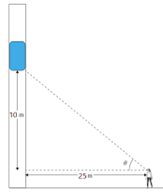
\includegraphics{../images/t1w1q1.png}
    \end{figure}
    
    Find the rate at which \(\theta\), the angle of elevation, is increasing when the elevator floor is 10m above Sarah’s eye level.

    \item 
    When a conical bottle rests on its flat base, the water in the bottle is 8 cm from its vertex.

    When the same conical bottle is turned upside down, the water level is 2 cm from its base.

    What is the height of the bottle?
    \begin{figure}[h]
        \centering
        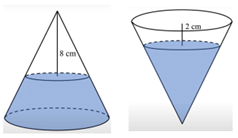
\includegraphics{../images/t1w1q2.png}
    \end{figure}
    
    \item 
    If \(x^5=1\), find the sum of \(\frac{x}{1+x^2}+\frac{x^2}{1+x^4}+\frac{x^3}{1+x}+\frac{x^4}{1+x^3}\)
\end{enumerate}

\end{document}